\documentclass{standalone}

\usepackage{tikz}

\usetikzlibrary{positioning, chains, shapes.geometric, fit, shapes, arrows.meta, calc}

\begin{document}

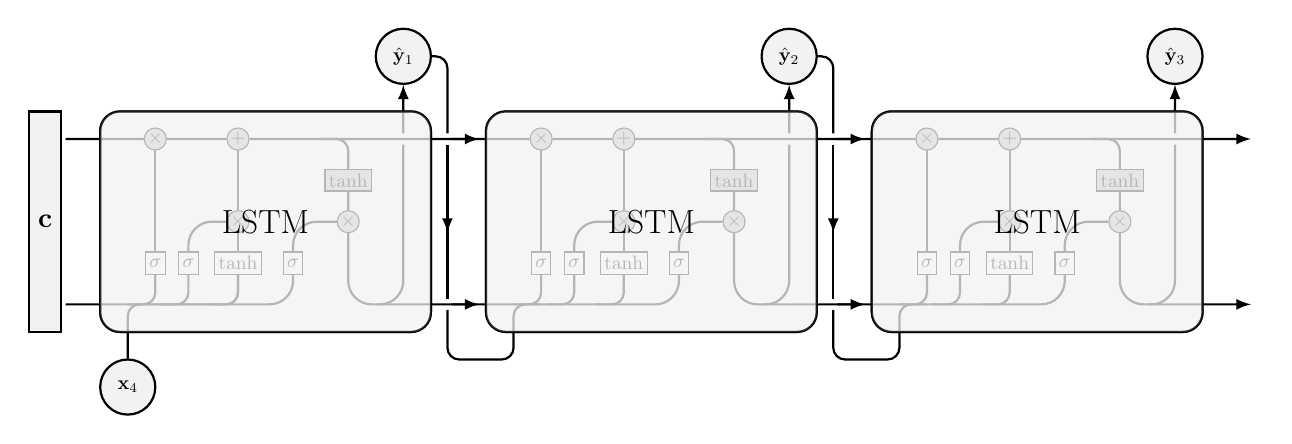
\begin{tikzpicture}[
    % GLOBAL CFG
    >=LaTeX,
    % Styles
    cell/.style={% For the main box
        rectangle, 
        rounded corners=2.5mm, 
        draw,
        thick,
        },
    operator/.style={%For operators like +  and  x
        circle,
        draw,
        inner sep=-0.5pt,
        minimum height =.4cm,
        align=center,
        fill=gray!50,
        },
    function/.style={%For functions
        rectangle,
        draw,
        inner sep=2pt,
        align=center,
        fill=gray!50,
        },
    ct/.style={% For external inputs and outputs
        },
    gt/.style={% For internal inputs
        rectangle,
        draw,
        inner sep=2pt,
        minimum height = 0.4cm,
        align=center,
        },
    ArrowC1/.style={% Arrows with rounded corners
        rounded corners=.15cm,
        thick,
        },
    ArrowC2/.style={% Arrows with big rounded corners
        rounded corners=.3cm,
        thick,
        },
    ]
% Define a macro for the LSTM cell
\newcommand{\LSTMCell}[3]{
    \node [cell, minimum height=4cm, minimum width=6cm] at (0,0){} ;
    % Draw inputs named ibox#
    \node [gt] (ibox1) at (-2,-0.75) {$\sigma$};
    \node [gt] (ibox2) at (-1.4,-0.75) {$\sigma$};
    \node [gt] (ibox3) at (-0.5,-0.75) {$\tanh$};
    \node [gt] (ibox4) at (0.5,-0.75) {$\sigma$};
   % Draw opérators   named mux# , add# and func#
    \node [operator] (mux1) at (-2,1.5) {$\times$};
    \node [operator] (add1) at (-0.5,1.5) {+};
    \node [operator] (mux2) at (-0.5,0) {$\times$};
    \node [operator] (mux3) at (1.5,0) {$\times$};
    \node [function] (func1) at (1.5,0.75) {$\tanh$};
    % Draw External inputs? named as basis c,h,x
    \node[] (c) at (-3.75,1.5) {};
    \node[] (h) at (-3.75,-1.5) {};
    \if#2y
        \node[circle, draw, minimum width=1cm, thick, align=center, fill=gray!10] (x) at (-2.5,-3) {$\mathbf{x}_{4}$};
    \fi
    \if#2n
        \node[] (x) at (-2.5,-3) {};
    \fi
    % Draw External outputs? named as basis c2,h2,x2
    \node[] (c2) at (4,1.5) {};
    \node[] (h2) at (4,-1.5) {};
    \node[circle, draw, minimum width=1cm, thick, align=center, fill=gray!10] (x2) at (2.5,3) {$\hat{\mathbf{y}}_{#1}$};
% Start connecting all.
    %Intersections and displacements are used. 
    % Drawing arrows    
    \draw [-latex, ArrowC1] (c) -- (mux1) -- (add1) -- (c2);
    % Inputs
    \draw [ArrowC2] (h) -| (ibox4);
    \draw [ArrowC1] (h -| ibox1)++(-0.5,0) -| (ibox1); 
    \draw [ArrowC1] (h -| ibox2)++(-0.5,0) -| (ibox2);
    \draw [ArrowC1] (h -| ibox3)++(-0.5,0) -| (ibox3);
    \if#2y
        \draw [ArrowC1] (x) -- (x |- h)-| (ibox3);
    \fi
    % Internal
    \draw [-, ArrowC2] (ibox1) -- node[midway, left] {} (mux1);
    \draw [-, ArrowC2] (ibox2) |- node[midway, xshift=-1.5, yshift=1.5] {} (mux2);
    \draw [-, ArrowC2] (ibox3) -- node[midway, xshift=12, yshift=1.5] {} (mux2);
    \draw [-, ArrowC2] (ibox4) |- node[midway, xshift=-1.5, yshift=1.5] {} (mux3);
    \draw [-, ArrowC2] (mux2) -- (add1);
    \draw [-, ArrowC1] (add1 -| func1)++(-0.5,0) -| (func1);
    \draw [-, ArrowC2] (func1) -- (mux3);
    %Outputs
    \draw [-latex, ArrowC2] (mux3) |- (h2);
    \draw (c2 -| x2) ++(0,-0.1) coordinate (i1);
    \draw [-, ArrowC2] (h2 -| x2)++(-0.5,0) -| (i1);
    \draw [-latex, ArrowC2] (i1)++(0,0.2) -- (x2);
    % Draw arrow to next cell if requested
    \if#3y
        \draw [ArrowC1] (x2) -| ++(0.8,-1.4);
        \draw [-latex, ArrowC1] (x2) ++(0.8,-1.6) -- ++(0,-1.6);
        \draw [ArrowC1] (x2) ++(0.8,-3) -- ++(0,-1.4);
        \draw [ArrowC1] (x2) ++(0.8,-4.6) |- ($(h2)+(0,-1)$);
        \draw [ArrowC1] ($(h2)+(0,-1)$) -| ($(h2)+(0.5,-0.5)$);
        \draw [ArrowC1] ($(h2)+(0.5,-0.5)$) |- ($(h2)+(1,0)$);
    \fi

    \node[cell, draw, fill=gray!10, opacity=0.75, minimum height=4cm, minimum width=6cm] at (0,0) {};
    \node[font=\LARGE] at (0,0) {LSTM};
}
% Use the LSTMCell macro three times with scaling
\begin{scope}[scale=0.7, transform shape, shift={(-8,0)}]
    \LSTMCell{1}{y}{y}
\end{scope}
\begin{scope}[scale=0.7, transform shape, shift={(-1,0)}]
    \LSTMCell{2}{n}{y}
\end{scope}
\begin{scope}[scale=0.7, transform shape, shift={(6,0)}]
    \LSTMCell{3}{n}{n}
\end{scope}

% Add the context vector block
\node[rectangle, draw, thick, minimum height=2.8cm, minimum width=0cm, fill=gray!10] (context) at (-8.4,0) {$\mathbf{c}$};

\end{tikzpicture}

\end{document}